\documentclass[text07.tex]{subfiles}
\begin{document}
%
% section 6.3
%
\section{HTMLについて}
\refstepcounter{PagePtr}\label{P:HTML}
% \refstepcounter{Exercise}

%
% section 6.3.1
%
\subsection{HTMLの復習\label{E:HTML}}

\bigskip

{\bfseries 考え方}

第１回で作成した\ruby{自己紹介}{じこしょうかい}ページのタグや機能を理解することでHTMLについて自分の思ったとおりに作れるようになりましょう。



HTMLは、タグという一つの機能をつかい、ウェブページを作り出します。\newline
タグというのは、{\textless}{\textgreater}{\textless}/{\textgreater}という形です。見覚えのある形ですね。\newline
例えば、

\ \ {\textless}p{\textgreater}文章をここに書きます。{\textless}/p{\textgreater}

のようなタグをpタグと\ruby{呼}{よ}びます。pタグはタグの間にある文章を表示します。\newline
まずは、第1回目の授業でみさなんが作成した自己紹介ページとその画像のファイルを第6回のフォルダにコピーし、それをmousepadでhtmlファイルを開いて見ましょう。

\begin{minipage}[b]{0.8\textwidth}
	\begin{enumerate}
		% \begin{minipage}[b]{1.5\textwidth}
			\item \ \ cp \ \ {\textasciitilde}/01/self\_intro.html \ \ \ {\textasciitilde}/06/www/index.html\\
			\ \ cp \ \ {\textasciitilde}/01/face.png \ \ \ {\textasciitilde}/06/www/\\
			cpコマンドを使って、 自己紹介ページのhtmlと<img src="face.png" などimgタグで指定している画像ファイルを、 第6回のwwwディレクトリにコピーしましょう。"face.png"以外にも使っている画像ファイルがあればコピーしてください。\\
			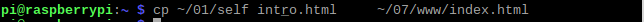
\includegraphics[width=14.73cm]{../../asset/image/ome7-img033.png}
			\bigskip
		% \end{minipage}

		\bigskip
		
		\item

		      \ \ cd \ \ {\textasciitilde}/06/www/\newline
		      cdコマンドを使って、（cpコマンドとは\ruby{違}{ちが}うよ。) 第6回のwwwディレクトリに\ruby{移動}{いどう}。


		\item \ \ mousepad index.html

		      \ \ mousepadでコピーした自己紹介のhtmlを開いてみよう。
		\begin{center}
			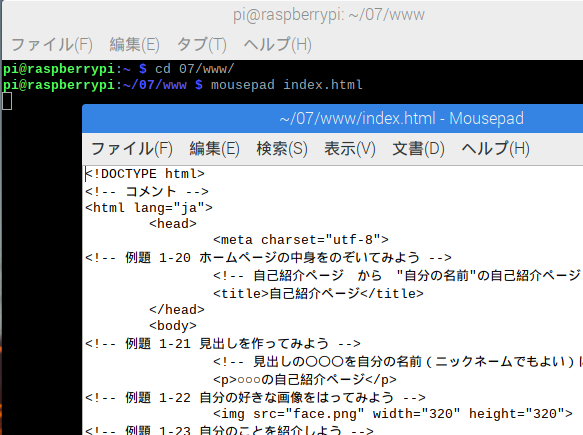
\includegraphics[width=0.8\textwidth]{../../asset/image/ome7-img034.png}
		\end{center}

	\end{enumerate}
\end{minipage}


開いたhtmlファイルの中に、実際にはウェブページに出てこない文章がちらほら見えます。

\ \ \ \ \ \ {\textless}!-{}- コメント -{}-{\textgreater}

それは、コメントという機能でウェブページには表示されない、メモのような機能でプログラムを書くときにあると便利です。HTMLに限らずHSPや様々なプログラム言語、はたまた現実世界でもメモというのは大切なので必要な情報はしっかりと書いておきましょう。

self\_intro.html内に使われたタグをまとめました。これを参考に自己紹介ページをより良くしていきましょう。

\clearpage

HTMLまとめ\\

\begin{table}[htbp]
	\centering
	% \caption{文字タイプ表}
	\begin{tabular}{|l|l|}
	\hline
        タグ名& \ruby{効果}{こうか}\\
		\hline

		{\textless}title{\textgreater}{\textless}/title{\textgreater} &ウェブページのタイトルをつける  \\
		\hline

		{\textless}h1{\textgreater}{\textless}/h1{\textgreater}&見出し(h1～h6)まで使える。h1が一番大きい \\
		\hline

		{\textless}ul{\textgreater}{\textless}/ul{\textgreater}&点付のリスト。リストの\ruby{項目}{こうもく}はliを使って表す  \\
		\hline

		{\textless}li{\textgreater}{\textless}/li{\textgreater}& リストの項目。ulもしくはolタグなどの中で使う \\
		\hline
        
        {\textless}p{\textgreater}{\textless}/p{\textgreater}&
        \begin{tabular}{l}
        \ruby{段落}{だんらく}を作るために使う。文字を表示したいときはこれを使う。\\
        改行は自動で行われるので自分のタイミングで行いたいときは{\textless}br{\textgreater}を\\
        使う  
		\end{tabular}\\
        \hline

		{\textless}br{\textgreater}&改行。pの中でも使うことができる  \\
		\hline

        {\textless}i{\textgreater}{\textless}/i{\textgreater}& イタリック（少し\ruby{傾}{かたむ}いた感じの文字） \\
		\hline

		{\textless}u{\textgreater}{\textless}/u{\textgreater}& 文字の下に線を引くときに使う \\
		\hline

        {\textless}a href=””{\textgreater}{\textless}/a{\textgreater}& 
        \begin{tabular}{l}
        リンクを貼りたいときに使う。\\
        hrefにはクリックしたときに飛びたいURLを入れる。
        \end{tabular}\\
		\hline

		{\textless}img src=””{\textgreater}& 
        \begin{tabular}{l}
        画像を表示するときに使用する。srcには画像の場所を指定する。\\
        ラズベリーパイの中の画像を指定しても、\\
        URLとして指定しても良い。 
        \end{tabular}\\
		\hline

        {\textless}ol{\textgreater}{\textless}/ol{\textgreater}& 
        \begin{tabular}{l}
        番号付きのリスト. liでリストの項目を決める。 \\
        番号はliの書いた順番通りになる
        \end{tabular}\\
		\hline

	\end{tabular}
  \end{table}

\bigskip

HTMLで使いたい色を探すときにはここを使うと便利です。

\url{https://www.colordic.org/m/}\newline
地下鉄のシンボルカラーとカラーコードで使いたい色がわかるはずです。

\url{https://www.colordic.org/}\newline
色の名前とカラーコードがわかります。色がまんべんなくあります。

\url{https://tech-unlimited.com/color.html}\newline
上級者向け、色の三原色というものから実際にHTML用のカラーコードに変えるサイトです。

\clearpage


また、HTMLにはボタンや文字を書き込む部分も作れます。\newline
通常見るだけのウェブページだったものがデータの送受信を可能とするなど、可能性を広げられます。

一部のタグを下に\ruby{記載}{きさい}します。

\begin{table}[htbp]
\centering
% \caption{文字タイプ表}
\begin{tabular}{|l|l|}
    \hline
    \begin{tabular}{l}
        {\textless}form{\textgreater}{\textless}/form{\textgreater}\\
        (使用例)\\
        {\textless}form action=”cgi-bin/formmail.cgi” {\textgreater}
    \end{tabular}
    &
    \begin{tabular}{l}
        入力送信フォームを作成\\
        formタグの中に
	    {\textless}input{\textgreater},
	    {\textless}select{\textgreater},\\
	    {\textless}textarea{\textgreater}
	    などをいれることで\\
	    ボタンや文字入力欄を作れる
    \end{tabular}
    \\ \hline 

    \begin{tabular}{l}
        {\textless}input{\textgreater}{\textless}/input{\textgreater}\\
	    (使用例)\\
	    {\textless}input type=”password” name=”pass”{\textgreater} 
    \end{tabular}

    &
    \begin{tabular}{c}
    文字の入力や、ボタンなどを作成するタグ。\\
    inputの次にtypeなどの\ruby{属性}{ぞくせい}を入れることで\\
    一行の文章やパスワードの入力などを決定する
    \end{tabular}
    \\\hline
\end{tabular}
\end{table}


それでは、formを使った例題を解いてみましょう。

例題\newline
自己紹介ページの一番下から2行上あたりにある{\textless}/body{\textgreater}の上の行から{\textless}form{\textgreater}タグで文字の入力をし、送信ボタンを\ruby{押}{お}せる機能を書きましょう。

{\bfseries 考え方}\newline
はじめに、formタグの間（{\textless}form{\textgreater}
＊＊ここ＊＊{\textless}/form{\textgreater})に、inputタグでテキストボックスを作る。そして、同じようにinputタグを使って送信ボタンという名前のボタンを作成する。

\begin{enumerate}
  \item
    \begin{wrapfigure}{r}{0.9\textwidth}
      \vspace{-\baselineskip}
      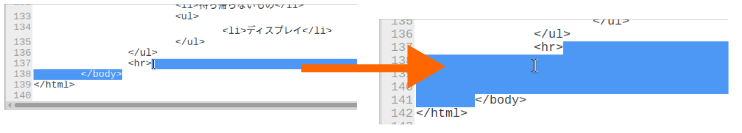
\includegraphics[width=\linewidth]{../../asset/image/ome7-img035.png}
    \end{wrapfigure}%
    {\textless}form{\textgreater}{\textless}/form{\textgreater}を書き込めるスペースを作ろう。

  \item
    \begin{wrapfigure}{r}{0.9\textwidth}
      \vspace{-\baselineskip}
      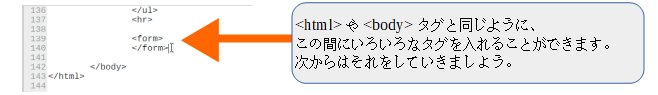
\includegraphics[width=\linewidth]{../../asset/image/ome7-img036.png}
    \end{wrapfigure}%
    {\textless}form{\textgreater}タグを書き足そう。

  \item
    \begin{wrapfigure}{r}{0.9\textwidth}
      \vspace{-\baselineskip}
      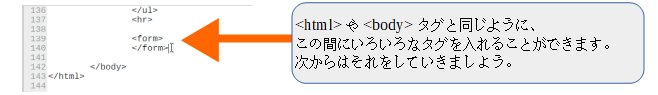
\includegraphics[width=\linewidth]{../../asset/image/ome7-img036.png}
    \end{wrapfigure}%
    {\textless}form{\textgreater}タグの間に、行を作り「テキストボックス」という文字が出るようにしよう。\\
    \ \ {\textless}form{\textgreater}\\
    \ \ \ \ \textbf{{\textless}p{\textgreater}テキストボックス{\textless}/p{\textgreater}}\\
    \ \ {\textless}/form{\textgreater}

\clearpage

  \item
    \begin{wrapfigure}{r}{0.9\textwidth}
      \vspace{-\baselineskip}
      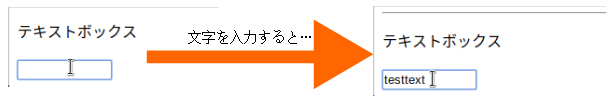
\includegraphics[width=\linewidth]{../../asset/image/ome7-img037.png}
    \end{wrapfigure}%
    次の行に{\textless}input{\textgreater}タグを入れよう。その際に、テキストを書き込めるようにしよう。\\
    \ \ 画像のようにするためには、\\
    \ \ {\textless}form{\textgreater}\\
    \ \ \ \ {\textless}p{\textgreater}テキストボックス{\textless}/p{\textgreater}\\
    \ \ \ \ \textbf{{\textless}input\ type="text"\ size="10"{\textgreater}}\\
    \ \ {\textless}/form{\textgreater}

  \item
    同じようなやり方で、先に書いた{\textless}input{\textgreater}タグから改行して次の行に{\textless}input{\textgreater}タグで送信ボタンを作成しよう。\\
    \ \ \ \ \textbf{{\textless}input type="submit" value="送信"{\textgreater}}

  \item
    作成したHTMLファイルを保存し、実際にブラウザで作成されているか確認してみましょう。\\
    このように、formタグ、inputタグには便利な機能があります。\\
    次の表に、inputタグの属性を一部記載しておきますので、\textbf{参考にして}問題を解いていきましょう。
\end{enumerate}

\clearpage

\begin{tcolorbox}[title=\useOmetoi,breakable]\label{Q:HTML}
  \begin{enumerate}
    \addex{最初に書いたテキストボックスの属性をパスワード入力ボックスに書き換えてみましょう。}
	  \addex{食べ物の名前を{\textless}p{\textgreater}タグを使って３つ追加してその横にチェックボックスを置きましょう。}
	  \addex{リセットボタンを送信ボタンの次の行に追加してみましょう。}
  \end{enumerate}
\end{tcolorbox}

\clearpage
% \refstepcounter{Question}\theQuestion\label{Q:HTML}\newline

% % 問題7-7　　
% \begin{enumerate}
% 	\item 最初に書いたテキストボックスの属性をパスワード入力ボックスに書き換えてみよう。
% 	\item 食べ物の名前を{\textless}p{\textgreater}タグを使って３つ追加してその横にチェックボックスを置きましょう。
% 	\item リセットボタンを送信ボタンの次の行に追加してみよう。
% \end{enumerate}

% \samepage

わからなかったら、先生に質問をすること。その間は\ruby{一覧}{いちらん}を見て考えてみよう。

inputタグの機能になるもの

\begin{table}[htbp]
	% \centering
	% \caption{文字タイプ表}
	\begin{tabular}{|c|l|}
	\hline
  type=”text” &
  \begin{tabular}{l}
    １行のテキストボックスを作ります。\\
    sizeの属性を指定することで大きさも決定できる。
  \end{tabular}\\ \hline

  type=”password” &
  \begin{tabular}{l}
    パスワード用のテキストボックスを作ります。\\
    入力されたら＊のマークなどに置き換わります。\\
    送信する際には\ruby{普通}{ふつう}の文字で送られるのに注意。
  \end{tabular}\\ \hline

  type=”checkbox” &
  \begin{tabular}{l}
    チェックボックスを作ります。\\
    複数\ruby{選択}{せんたく}可能で、checked属性を指定すると\\
    予めチェックが入ったかどうかを決めれる。
  \end{tabular}\\ \hline 

  type=”radio” &
  \begin{tabular}{l}
    ラジオボタンを作ります。複数の中から１つしか選択できないのが\ruby{特徴}{とくちょう}。\\
    こちらもcheckedで\ruby{状態}{じょうたい}を決めれる。
  \end{tabular}\\ \hline 

  type=”submit” &
  \begin{tabular}{l}
    送信ボタンを作ります。
  \end{tabular}\\ \hline 

  type=”button” &
  \begin{tabular}{l}
    普通のボタンを作ります。
  \end{tabular}\\ \hline 

  type=”image” &
      \begin{tabular}{l}
        画像のボタンを作ります。\\
        使用する画像ファイルは、src属性で指定しましょう。\\
        またalt属性が\ruby{必須}{ひっす}。
      \end{tabular}\\ \hline 

  type=”reset” &
      \begin{tabular}{l}
        リセットボタンを作ります。\\
        このボタンを押すと、書いていたデータがなくなり\\
        最初の状態に\ruby{戻}{もど}ります。
      \end{tabular}\\ \hline 
		
	\end{tabular}
\end{table}

\clearpage\end{document}
